\section{Method}
To make a bird recognition program two main procedures are required. First a feature
extraction method that can analyze and extract the desired features from a
sound file of a bird singing and secondly a decision making algorithm that can
take the extracted features and classify a bird. The method choosen feature
extraction was Periodogram which evalutes the power spectral density of the
input signal and CBR was used for the classification.

\begin{figure}[h]
\centering
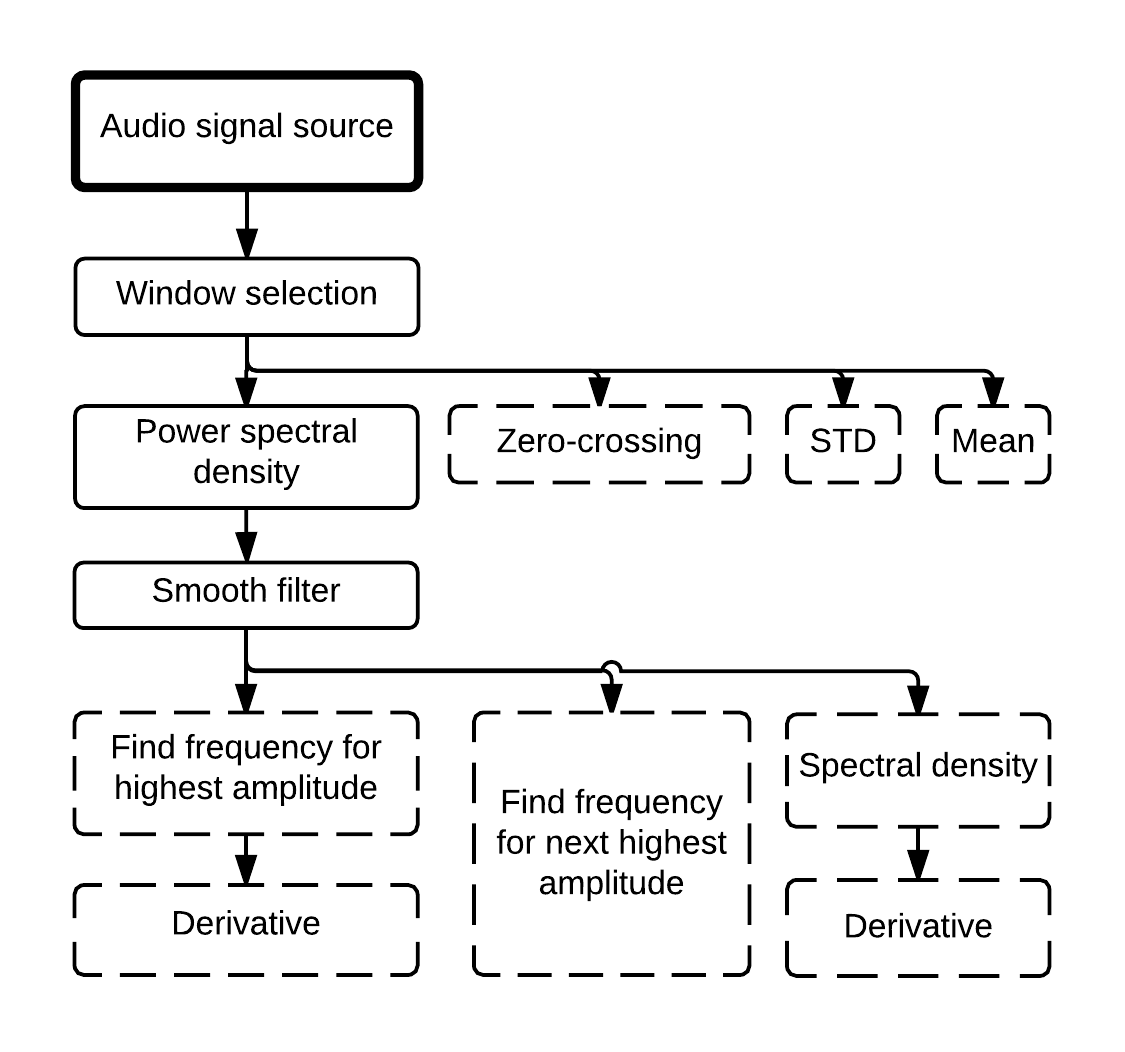
\includegraphics[width=0.5\textwidth]{feature_tree2}
\caption{Overall approach. Audio signal is the source of all information. The normal lines are transforming data and the dashed lines are the features being used.}
\label{fig:approach}
\end{figure}

\subsection{Feature extraction}
Given an audio signal recordning of a bird, it is important for the feature extraction
procedure to extract unique set of features that can be used for identity recognition.
In order to achieve this, the Matlabs Periodogram function was used to calculate the power
spectral density in contemplation of extracting the influential features from the audio signal.

As shown in Figure~\ref{fig:scanningWindow} a window with a predifined
length scans the original audio signal. The power spectral density of the window
is calculated and the results are visualized in Figure~\ref{fig:periodogram}.
The highest peaks from the power spectral density shown in Figure~\ref{fig:periodogram_peaks} were found
by using the Matlabs FindPeaks function. These peaks are used as features and additional feature extraction shown in Figure~\ref{fig:approach}.

The described procedure is repeated for each audio recording file.

\begin{figure}[htp]
    \subfloat[A window scanning the original audio recording.]{
      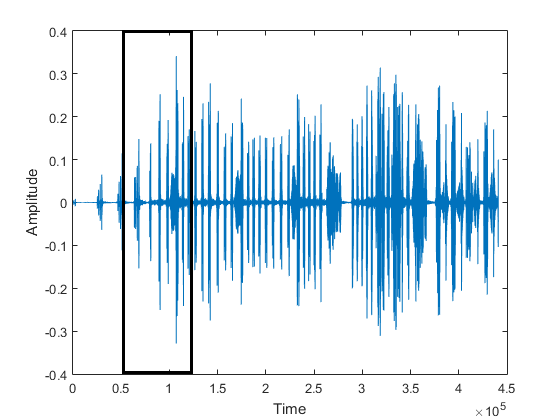
\includegraphics[clip,width=\columnwidth]{audio}
      \label{fig:scanningWindow}
    }

    \subfloat[The power spectral density of a single window.]{
      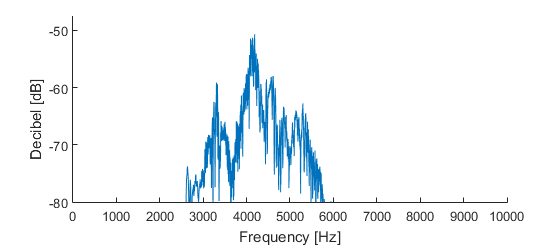
\includegraphics[clip,width=\columnwidth]{periodogram}
      \label{fig:periodogram}
    }

    \subfloat[Peaks with the highest amplitude in the power spectral density.]{
      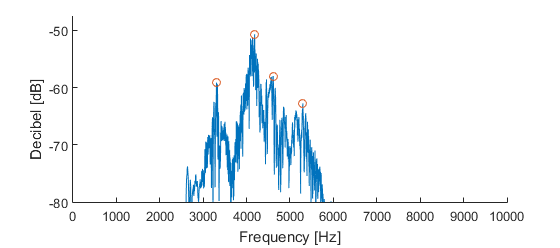
\includegraphics[clip,width=\columnwidth]{periodogram_peaks}
      \label{fig:periodogram_peaks}
    }

    \subfloat[Stored peaks over time.]{
      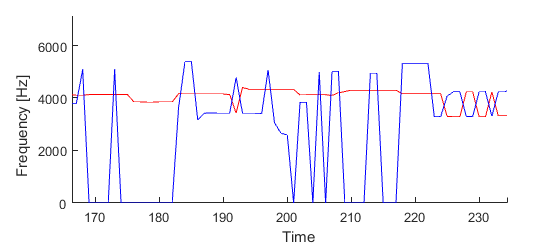
\includegraphics[clip,width=\columnwidth]{peaks_over_time}
      \label{fig:peaks_over_time}
    }

    \caption{Feature extraction procedure is devided into three parts.}
    \label{fig:featureExtraction}
\end{figure}



\subsection{Case matching algorithm}
The class and the features
(Class, FFT Area, FFT Area Delta, FFT Peak 1, FFT Peak 2, FFT Peak 1 Delta, Mean, STD, ZCR)
are stored row-wise in a file. This will be the database of cases.
The class Bluethroat2 is removed from the database and put into another file, that will be the sample file.

The input of kNN is the database features, sample features, k value, distance type, wieghts.
Each sample features are compared with the database using a distance function (Eeucledian, Manhattan, Canberra).
The output of kNN is the estimated class.
If there is a equal amount of class inside the circle it will output unknown class.

\begin{figure}[htp]
    \subfloat[Two samples evaluates to four black and four gray. The probobility of being the black or white class is 50.
    It is likily that this is unknown class. A unkown class can be pervieved as either noisy sample or listening to more than one type of bird at the same time.]{
      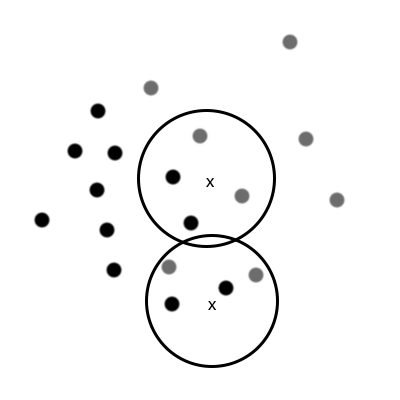
\includegraphics[clip,width=\columnwidth]{knna}
    }

    \subfloat[Three samples evaluates to seven black and five gray. The probobility to being the black class is over 50.]{
      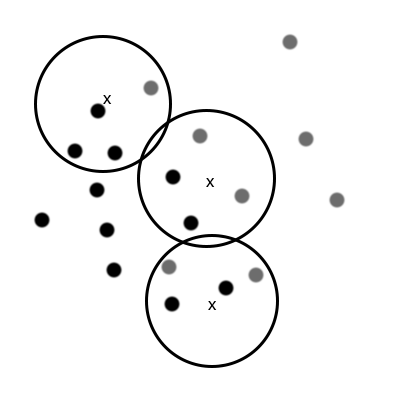
\includegraphics[clip,width=\columnwidth]{knnb}
    }

    \caption{This shows how more samples can increase the accuracy. kNN evaluation where k = 4. Evaluates to the class which has the greater number of class inside the circle.}
    \label{fig:featureExtraction}
\end{figure}
